\documentclass{article}
\usepackage[margin=1in]{geometry}
\usepackage{graphicx}
\usepackage{caption}
\usepackage{subcaption}
\usepackage{amsmath}

\title{UNet Model with Monte Carlo Dropout for Image Segmentation}
\author{Mohamed Hasan}
\date{\today}

\begin{document}
\maketitle

\section{Introduction}
This report details the development and evaluation of a custom Artificial Neural Network (ANN) 
designed for image segmentation tasks. I focus on a UNet model architecture, built from scratch 
using TensorFlow 2, to perform segmentation on satellite images. To enhance the robustness and 
reliability of the model, I implement Monte Carlo (MC) Dropout as a method for uncertainty quantification. 
This approach allows me to assess the confidence of the model’s predictions, providing valuable 
insights into the reliability of segmentation results.

The experiments involve an evaluation of different activation functions, loss functions, and 
other hyperparameters, with a focus on their impact on uncertainty quantification. The satellite 
image dataset, comprising of a mix of real and synthetic images and corresponding masks, serves as 
a challenging real-world scenario due to factors like variable lighting conditions, diverse backgrounds, 
and the presence of objects (i.e. astroids).


\section{Dataset}
The dataset consists of satellite images and corresponding masks, with each mask delineating the
satellite from the background. The images are of varying resolutions and quality, reflecting the
diversity of satellite imagery encountered in real-world scenarios. The dataset is divided into
training and validation sets, with the training set containing 3116 images and the validation set
comprising 600 images. The masks are categorized into fine and coarse masks, with 403 fine masks
and 2114 coarse masks in the training set. The dataset presents a challenging segmentation task due
to the presence of complex textures, varying lighting conditions, and the need to accurately
delineate the satellite from the background.

\begin{figure}[h]
    \centering
    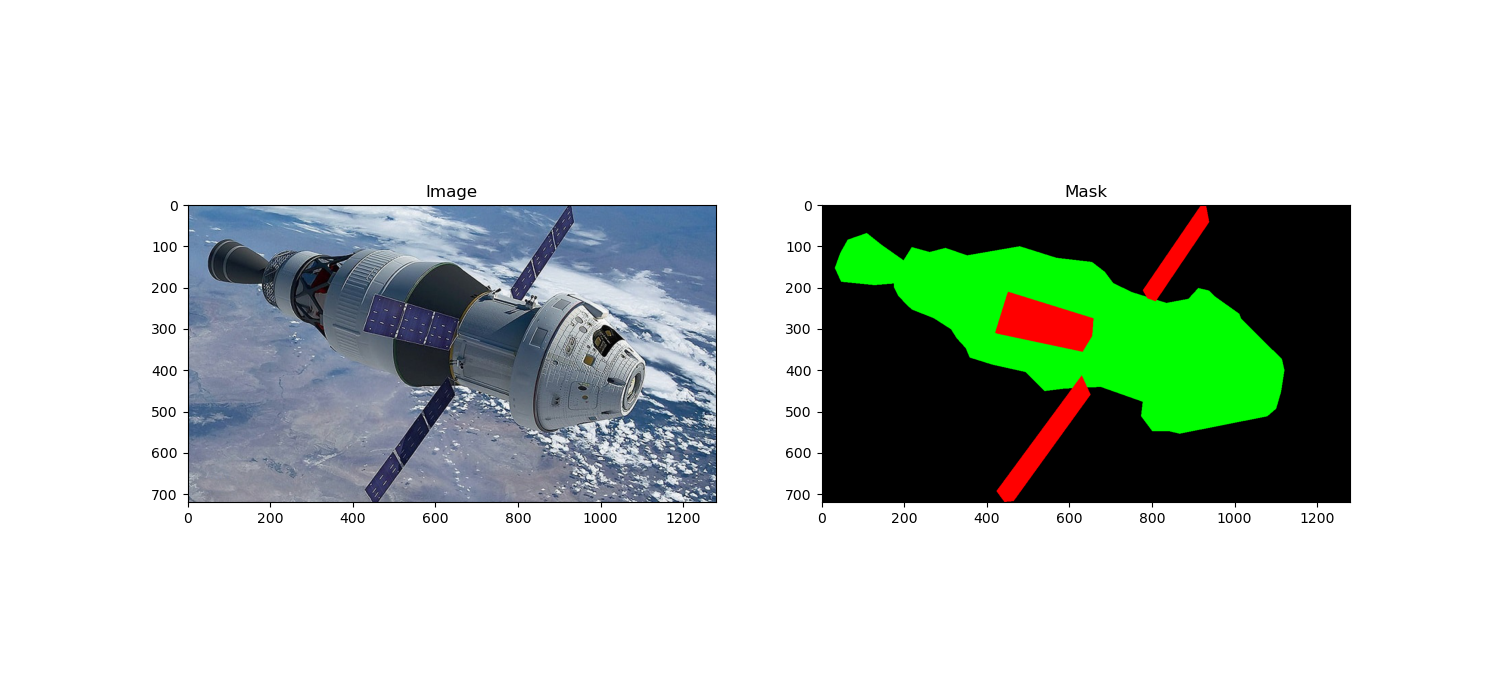
\includegraphics[width=0.7\textwidth]{../images/original_input_sample.png}
    \caption{Sample images and masks from the dataset.}
    \label{fig:dataset}
\end{figure}


\section{Setup}
I developed a custom UNet model for image segmentation using TensorFlow 2. The UNet architecture, 
known for its effectiveness in biomedical image segmentation, is adapted to handle the challenges 
of satellite imagery. The dataset comprises a mix of synthetic and real satellite images, each 
accompanied by a corresponding mask that delineates the satellite from the background.

\subsection{Training and Evaluation}

The training configuration involved using a combination of Binary Cross Entropy (BCE) and Dice Loss 
as the loss function. The BCE loss, given by

\[
\text{BCE} = -\frac{1}{N} \sum_{i=1}^{N} [y_i \log(p_i) + (1 - y_i) \log(1 - p_i)],
\]

where \( y_i \) is the ground truth label and \( p_i \) is the predicted probability, effectively 
handles the class imbalance inherent in segmentation tasks. The Dice Loss, formulated as

\[
\text{Dice Loss} = 1 - \frac{2 \sum_{i=1}^{N} y_i p_i}{\sum_{i=1}^{N} y_i + \sum_{i=1}^{N} p_i},
\]

complements the BCE loss by directly optimizing for the Dice Coefficient, a common metric in image 
segmentation.

To evaluate the model’s performance, I employed the Dice Coefficient and Accuracy as metrics. The 
dataset was divided into training and validation sets, with the training set comprising 3116 images 
(403 with fine masks and 2114 with coarse masks) and the validation set consisting of 600 images 
with fine masks.

The final model achieved a loss of 0.598, an accuracy of 0.868, and a Dice Coefficient of 0.646 on 
the validation set.

For uncertainty quantification, I implemented Monte Carlo (MC) Dropout. By incorporating dropout 
layers with a dropout rate of 0.35 during inference and performing multiple forward passes, I generated 
a distribution of predictions for each input image. This approach allowed me to compute the mean prediction 
and the standard deviation for each pixel, providing insights into the model’s confidence. The mean 
prediction is given by

\[
\mu(x) = \frac{1}{T} \sum_{t=1}^{T} \hat{y}_t(x),
\]

where \( \hat{y}_t(x) \) is the prediction at the \( t \)-th forward pass and \( T \) is the number of 
passes. The uncertainty is quantified as the standard 
deviation of these predictions,

\[
\sigma(x) = \sqrt{\frac{1}{T} \sum_{t=1}^{T} (\hat{y}_t(x) - \mu(x))^2}.
\]

This method enabled me to identify areas with high uncertainty, particularly around object boundaries 
and regions with complex textures.



\begin{figure}[h]
    \centering
    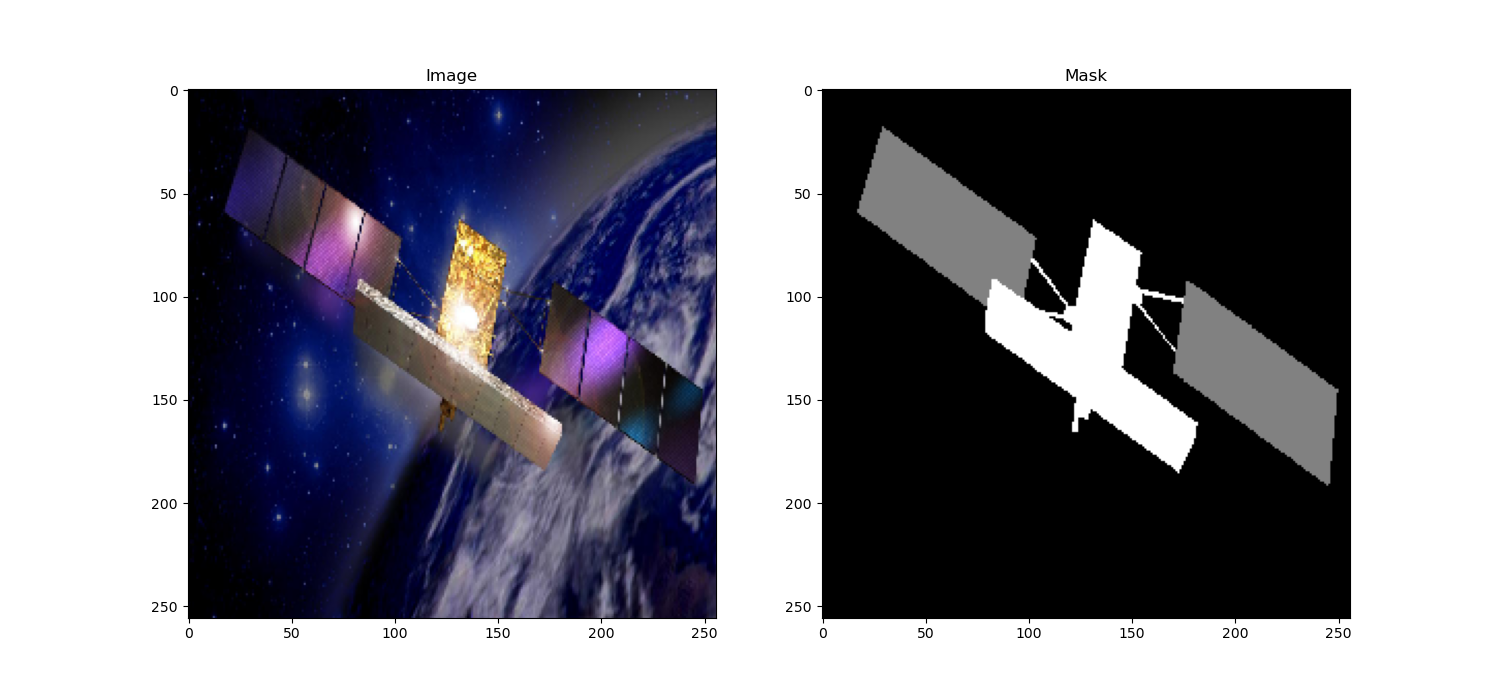
\includegraphics[width=0.7\textwidth]{../images/processed_input_sample.png}
    \caption{Setup and preprocessing of images and masks.}
    \label{fig:setup}
\end{figure}

\section{Monte Carlo Dropout}
\begin{itemize}
    \item Monte Carlo (MC) Dropout is used with a dropout rate of 0.35.
    \item Predict with dropout enabled: \texttt{model.predict(training=True)}
    \item Mean Prediction Image: Shows the predicted segmentation map. Brighter areas indicate higher confidence.
    \item Prediction Uncertainty Image (Standard Deviation): Shows variability in predictions across MC samples. Brighter areas indicate higher uncertainty.
\end{itemize}

\begin{figure}[h]
    \centering
    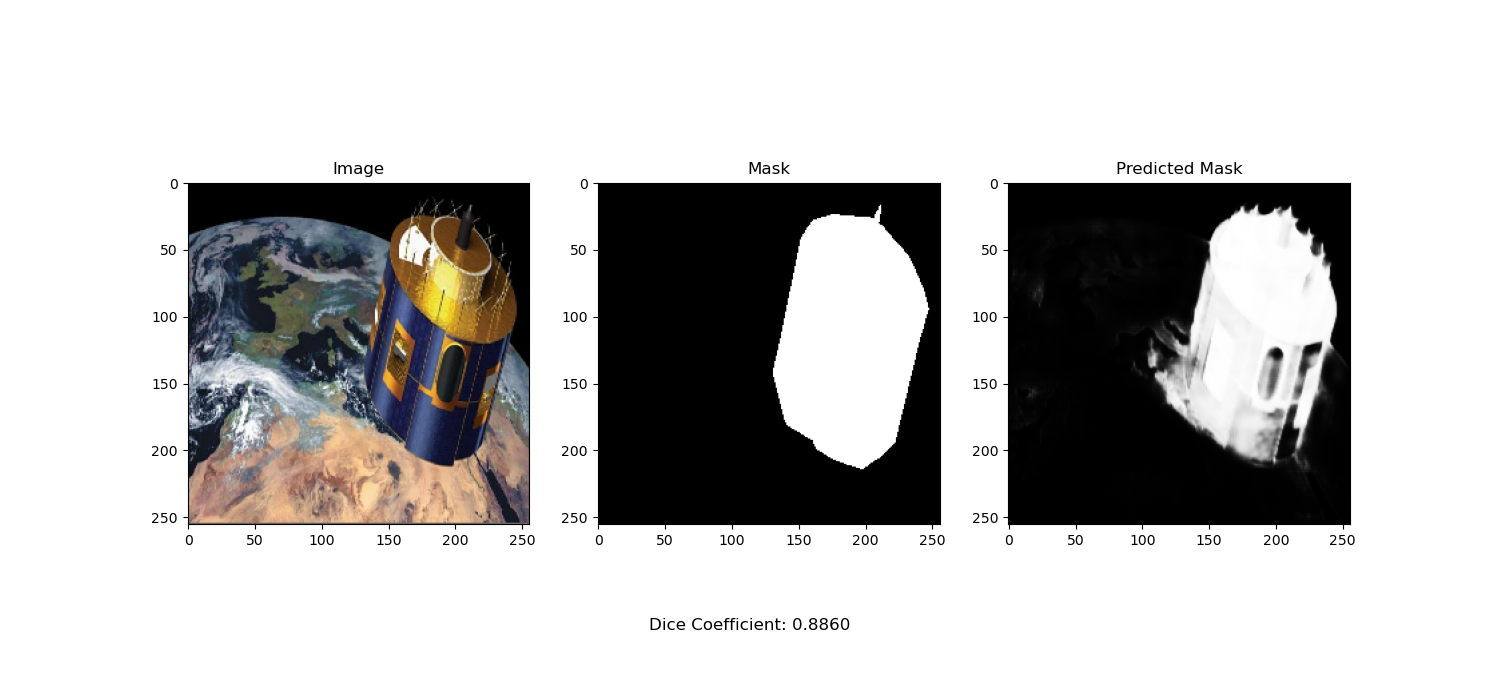
\includegraphics[width=0.7\textwidth]{../images/output_sample.png}
    \caption{MC Dropout predictions and uncertainties.}
    \label{fig:mc_dropout}
\end{figure}

\section{Results}
\subsection{Test Image 1}
\begin{itemize}
    \item Test Mask: Clear delineation of the satellite.
    \item Mean Prediction: Successfully captures the shape with some blurriness.
    \item Uncertainty: Higher around the edges, indicating lower confidence.
\end{itemize}

\begin{figure}[h]
    \centering
    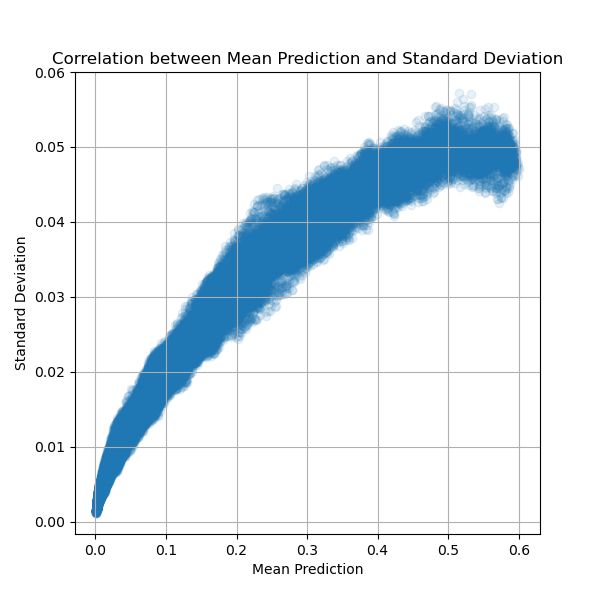
\includegraphics[width=0.8\textwidth]{../images/MC_dropout/all_test_image_correlation_between_mean_prediction_and_std.png}
    \caption{Results for Test Image 1.}
    \label{fig:result_1}
\end{figure}

\subsection{Test Image 2}
\begin{itemize}
    \item Test Mask: Well-defined satellite and solar panels.
    \item Mean Prediction: Captures the structure with some diffusion.
    \item Uncertainty: Concentrated around the edges of the solar panels.
\end{itemize}



\subsection{Test Image 3}
\begin{itemize}
    \item Test Mask: Complex structure with different parts.
    \item Mean Prediction: Approximates the shape but with less precision.
    \item Uncertainty: Higher in regions with intricate details.
\end{itemize}

\subsection{Test Image 4}
\begin{itemize}
    \item Test Mask: Small satellite with a backdrop of asteroids.
    \item Mean Prediction: Captures the satellite but with significant blurriness.
    \item Uncertainty: High around the satellite.
\end{itemize}


\subsection{Test Image 5}
\begin{itemize}
    \item Test Mask: Satellite with large solar panels.
    \item Mean Prediction: Shape captured with noticeable blurriness.
    \item Uncertainty: Elevated around the edges.
\end{itemize}


\section{Uncertainty Analysis}
\begin{itemize}
    \item Low Uncertainty Average: 0.0195
    \item Medium Uncertainty Average: 0.1598
    \item High Uncertainty Average: 0.0449
\end{itemize}

\section{Correlation Between Mean and Standard Deviation}
\begin{itemize}
    \item Horizontal Axis (Mean Prediction): Average prediction values.
    \item Vertical Axis (Standard Deviation): Standard deviation of predictions.
    \item Higher concentration of low standard deviations at extreme mean values.
    \item Spread in standard deviation for mean values around 0.4 to 0.6, indicating higher uncertainty.
\end{itemize}

\begin{figure}[h]
    \centering
    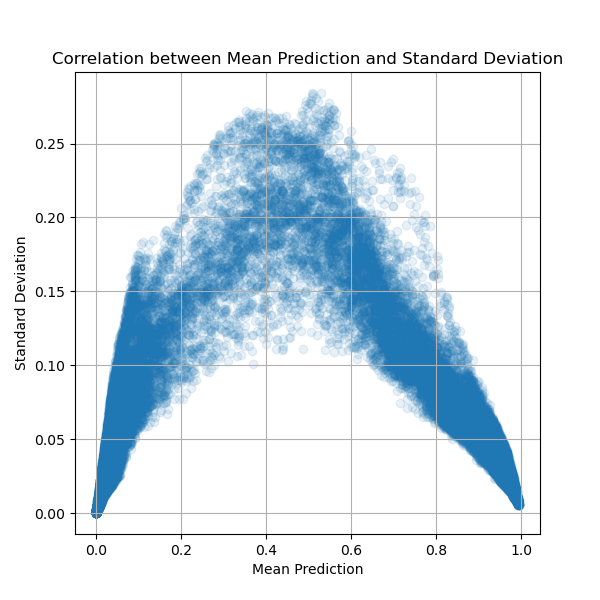
\includegraphics[width=0.8\textwidth]{../images/MC_dropout/test_image[0]_correlation_between_mean_prediction_and_std.png}
    \caption{Correlation between Mean Prediction and Standard Deviation.}
    \label{fig:correlation_analysis}
\end{figure}

\section{Conclusion}
The results illustrate the effectiveness of using MC dropout to estimate uncertainty in the model's predictions. The model performs well in capturing the general shapes of the satellites, but there is room for improvement in reducing the blurriness and increasing the precision of the predictions. Future work could focus on refining the model architecture or incorporating additional data augmentation techniques to enhance the model's performance and confidence.

\end{document}
